\subsection{BioPAX 3 Property Editor} \label{BioPAX_Property_Editor}
\textbf{Plugins$\Rightarrow$BiNoM BioPAX 3 Utils$\Rightarrow$ BioPAX 3 Property Editor}\\
All the information available in a BioPAX file can be easily retrieved using the BioPAX Property Editor function. A component on the diagram must be selected first (CDC2 in Figure \ref{BioPAX_Property_Editor_cdc2}) and a window appears with all available information concerning the molecule.\\\\
\begin{figure}[h]
\centering
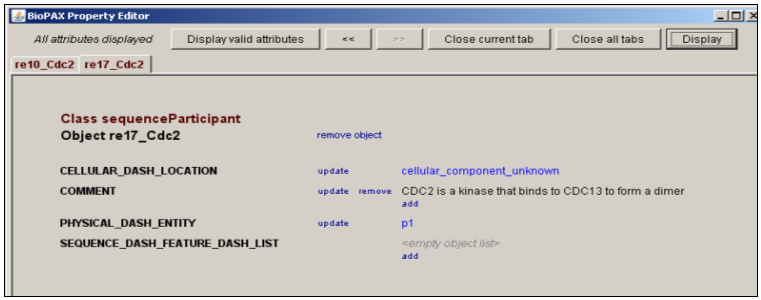
\includegraphics[width=0.8\textwidth]{graphics/BioPAX_Property_Editor_cdc2}
\caption{BioPAX Property Editor: example of the properties concerning CDC2 component in M-Phase model}
\label{BioPAX_Property_Editor_cdc2}
\end{figure}
\parbox{\textwidth}{ In the menu of the Property Editor, several options are offered:
\begin{itemize}
\item Display valid attributes / Display all attributes hides all the empty fields (for example, in Figure \ref{BioPAX_Property_Editor_apoptosis}: Availability or Evidence have \textless empty object list\textgreater and would be hidden) / shows all the available fields, even the empty ones.
\item  \textless\textless~and \textgreater\textgreater~correspond to back or forward buttons and follow the historical exploration of the Property Editor (similar to ‘Back’ and ‘Forward’ buttons of a network browser).
\item Close current tab or Close all tabs closes the current page of the property editor or all the open pages.
\item  Display / Edit shows a simple display of the page editor where no change can be made (Figure \ref{BioPAX_Property_Editor_apoptosis}) / allows changes in the fields by adding, removing or updating information (Figure \ref{BioPAX_Property_Editor_cdc2}). For the latter, click first on the Edit tab on the upper menu, then on update situated near the field to modify. In Figure \ref{BioPAX_Property_Editor_cdc2}, as an example, some comments were added manually: “CDC2 is a kinase that binds to CDC13 to form a dimer”. In the Apoptosis example (Figure \ref{BioPAX_Property_Editor_apoptosis}), extensive information is already available concerning the pathway, references, etc.
\end{itemize}}
\begin{figure}[h]
\centering
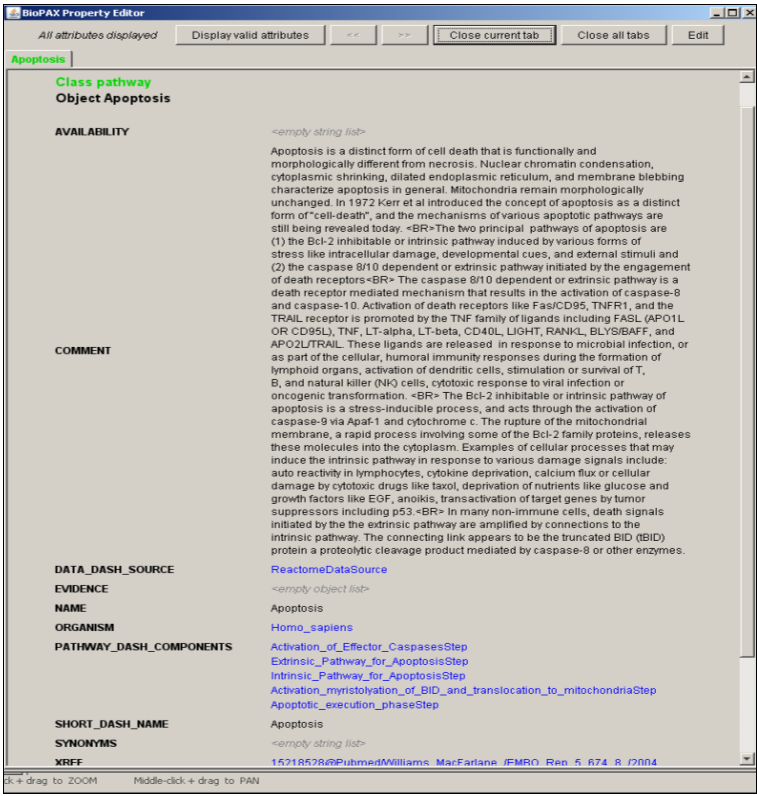
\includegraphics[width=0.8\textwidth]{graphics/BioPAX_Property_Editor_apoptosis}
\caption{BioPAX Property Editor: example of “apoptosis pathway” node properties}
\label{BioPAX_Property_Editor_apoptosis}
\end{figure}	
For more details on BioPAX description standard, visit the webpage: http://www.biopax.org/ 
\subsection{BioPAX 3 Class Tree}
\textbf{Plugins$\Rightarrow$BiNoM BioPAX 3 Utils$\Rightarrow$BioPAX 3 Class Tree}\\
All the statistics concerning the pathway are listed: the number of reactions, associations or catalyses, the number of proteins or complexes, etc (figure~\ref{BioPAX_Class_Tree}). More information can be accessed by selecting a specific object which, when clicked on, leads to the BioPAX 3 Property Editor window (see section~\ref{BioPAX_Property_Editor}).\\\\
\begin{figure}[h]
\centering
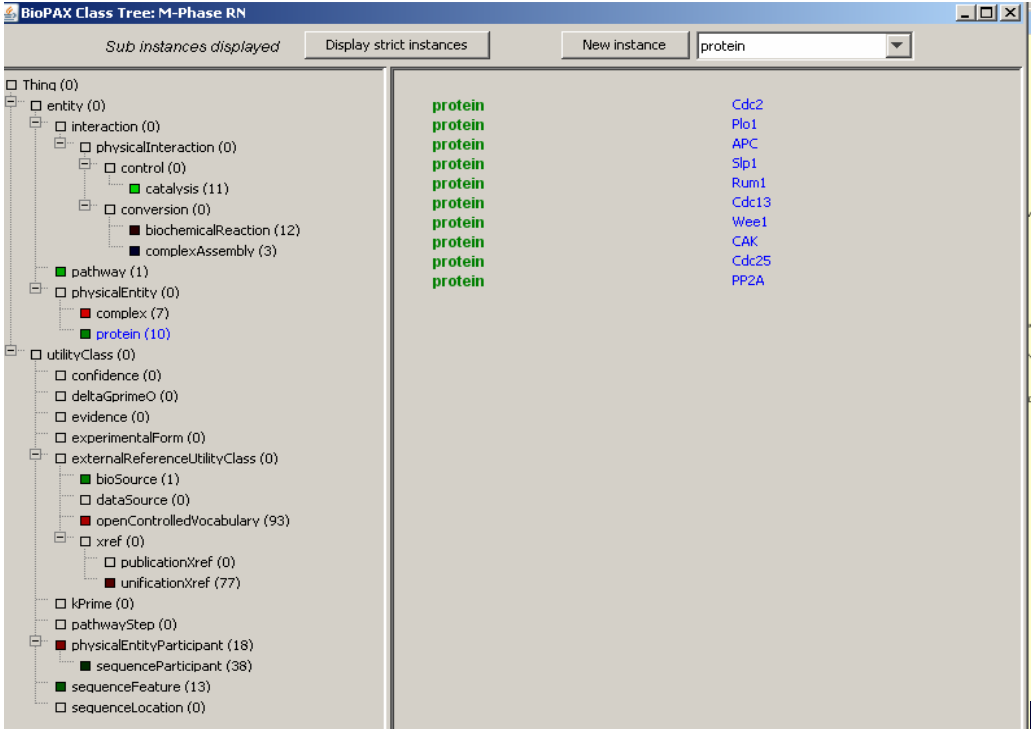
\includegraphics[width=0.8\textwidth]{graphics/BioPAX_Class_Tree}
\caption{BioPAX Class tree. On the left frame, the model is described in terms of interactions, entities, etc. On the right frame, the proteins, selected in the left frame, are listed. The links are clickable and open a BioPAX Property Editor window.}
\label{BioPAX_Class_Tree}
\end{figure}
To complete the network, the user can easily add new information or a new protein, protein complex, type of interaction, etc., by clicking on the New Instance tab.

\subsection{Use Simplified URI Names}
\textbf{Plugins$\Rightarrow$BiNoM BioPAX 3 Utils$\Rightarrow$Use Simplified URI Names}\\
In the BioPAX Class Tree, protein names can have either URI names (Uniform Resource Identifier used to give a unique identification to proteins) or “BiNoM Naming Service” names. For example, for the apoptosis pathway, the protein BAD is referred to as\\
“\textit{UniProt\_Q92934\_Bcl2\_antagonist\_of\_cell\_death\_BAD\_\_Bcl\_2\_binding\_component\_6\_\_Bcl\_\_XL\_Bcl\_2\\
\_associated\_death\_promoter\_\_Bcl\_2\_like\_8\_protein}”\\
in the URI case and just “BAD” in the BiNoM Naming Service case. For the rules of how BiNoM generates names see section~\ref{BiNoM_Naming_Service}.

\subsection{Synchronize networks with BioPAX 3}
\textbf{Plugins$\Rightarrow$BiNoM BioPAX 3 Utils$\Rightarrow$Synchronize networks with BioPAX 3}\\
This command updates all the interfaces according to the changes made to individual BioPAX objects.